

\fancypagestyle{miEstilo506}{
   \lhead{5.6 Descripción de archivos y directorios}
   \rhead{Página \thepage}
   \lfoot{}
   \cfoot{}
   \rfoot{}
}

\pagestyle{miEstilo506}


\subsection{Descripción de archivos y directorios}

La aplicación \texttt{SIVIRA} está compuesta por una serie de archivos y directorios que implementan y ejecutan el conjunto de servicios del sistema de videovigilancia.

Todos estos archivos y directorios están disponibles en el repositorio oficial del proyecto en Github \cite{ref1}.

\begin{figure}[h]
	\centering
	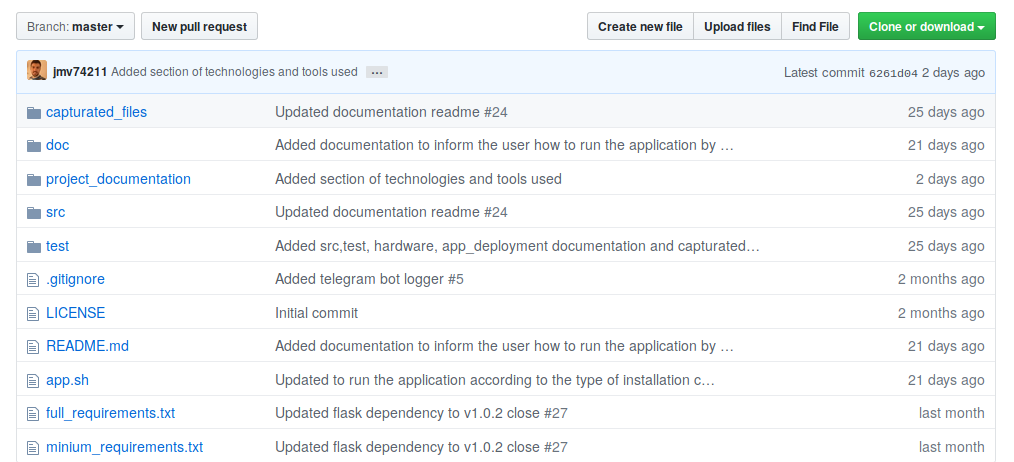
\includegraphics[scale=0.5]{images/43}
	\caption{Repositorio de Github del proyecto SIVIRA}
\end{figure}

A continuación, se explicará cómo se ha organizado todos estos archivos y directorios, junto con una breve descripción sobre el objetivo de cada uno.

\textbf{Capturated\_files}

Este directorio está destinado a almacenar el conjunto de archivos de imágenes y vídeo generados por el sistema de videovigilancia. Su estructura es la siguiente puede verse en la figura \ref{fig:tik1}.

Se compone de los siguientes elementos:

\vspace{-0.5cm}

\begin{itemize}
\item \textbf{alerts}: Directorio donde se almacenan todos los archivos generados mediante alertas (capturas o grabaciones automáticos tras ser activado el sensor de movimiento).

	\begin{itemize}
	\item \textbf{false\_positive}: Directorio donde serán almacenados todos los archivos generados tras ser activado el sensor de movimiento y que el agente detector de objetos ha filtrado tras comprobar que no hay ninguna persona en dichas fotos.
	\end{itemize}

\item \textbf{photos}: Directorio donde se almacenan todas las fotos capturadas de forma manual.

\item \textbf{videos}: Directorio donde se almacenan todas los vídeos capturados de forma manual.

\item \textbf{Readme.md}: Archivo de documentación para el repositorio.

\end{itemize}



\tikzstyle{every node}=[draw=black,thick,anchor=west]
\tikzstyle{selected}=[draw=red,fill=red!30]
\tikzstyle{optional}=[dashed,fill=gray!50]

\begin{figure}[H]
\centering

\begin{tikzpicture}[%
  grow via three points={one child at (0.5,-0.7) and
  two children at (0.5,-0.7) and (0.5,-1.4)},
  edge from parent path={(\tikzparentnode.south) |- (\tikzchildnode.west)}]
  \node {SIVIRA\_APP}
    child { node {capturated\_files}
		  child { node {alerts}
		  		child { node {false\_positive}}
		  }
		  child [missing] {}	
          child { node {photos}}
          child { node {videos}}
          child { node {README.md}}     
    }
    child [missing] {}	
    child [missing] {}	
    child [missing] {}	
    child [missing] {}	
    child [missing] {}	
    child { node {\ldots}};
   
\end{tikzpicture}
\caption{Estructura de directorios de capturated\_files} \label{fig:tik1}
\end{figure}

\textbf{Doc}

Este directorio contiene una estructura de archivos de documentación en formato \texttt{.md} para que puedan ser consultados desde el repositorio de Github. Su estructura es la siguiente puede verse en la figura \ref{fig:tik2}.

\begin{figure}
\centering
\begin{tikzpicture}[%
  grow via three points={one child at (0.5,-0.7) and
  two children at (0.5,-0.7) and (0.5,-1.4)},
  edge from parent path={(\tikzparentnode.south) |- (\tikzchildnode.west)}]
  \node {SIVIRA\_APP}
  	child { node {\ldots}}
    child { node {doc}
		  child { node {api}
		  		child { node {README.md}}
		  		child { node {api\_agent\_doc.md}}
		  		child { node {object\_detector\_agent\_doc.md}}
		  }
		  child [missing] {}
		  child [missing] {}
		  child [missing] {}
		  child [missing] {}	
          child { node {app\_deployment}
          		child { node {README.md}}
          }
          child [missing] {}
          child { node {backend\_app}
                child { node {README.md}}
          }
          child [missing] {}
          child { node {hardware}
                child { node {README.md}}
          }
          child [missing] {}
          child { node {images}
                child { node {\ldots}}
          }
		  child [missing] {}
          child { node {installation}
                child { node {README.md}}
          }  
		  child [missing] {}
          child { node {test}
                child { node {README.md}}
          }
          child [missing] {} 
		  child [missing] {}
          child { node {user\_guide}
                child { node {README.md}}
          }         
          child [missing] {}           
          child [missing] {}      
          child { node {README.md}}     
    }
    child [missing] {}	
    child [missing] {}	
    child [missing] {}	
    child [missing] {}	
    child [missing] {}
    child [missing] {}
    child [missing] {}
    child [missing] {}
    child [missing] {}
    child [missing] {}
    child [missing] {}
    child [missing] {}
    child [missing] {}
    child [missing] {}
    child [missing] {}
    child [missing] {}
    child [missing] {}
    child [missing] {}
    child [missing] {}
    child [missing] {}
    child [missing] {}
    child [missing] {} 
    child { node {\ldots}};

\end{tikzpicture}
\caption{Estructura de directorios de doc} \label{fig:tik2}
\end{figure}


Se compone de los siguientes elementos:

\vspace{-0.5cm}

\begin{itemize}
\item \textbf{api}: Directorio donde se almacena la documentación de la \texttt{API}.

	\begin{itemize}
	\item \textbf{README.md}: Documentación sobre aplicación y uso de la \texttt{API} y la api del agente detector de objetos.
	\item \textbf{api\_agent\_doc.md}: Documentación sobre aplicación y uso de la \texttt{API} principal.
	\item \textbf{object\_detector\_agent.md}: Documentación sobre aplicación y uso del agente detector de objetos.
	\end{itemize}

\item \textbf{app\_deployment}: Directorio que contiene documentación sobre cómo desplegar y ejecutar la aplicación.

\item \textbf{backend\_app}: Directorio que contiene documentación el contenido del directorio \textit{src}.

\item \textbf{hardware}: Directorio que contiene documentación sobre el hardware necesario, cómo instalarlo y su presupuesto.

\item \textbf{images}: Directorio que contiene las imágenes que se han utilizado en la documentación del repositorio.

\item \textbf{installation}: Directorio que contiene documentación sobre cómo instalar los componentes necesarios para ejecutar la aplicación.

\item \textbf{test}: Directorio que contiene documentación sobre cómo ejecutar los tests de la aplicación.

\item \textbf{user\_guide}: Directorio que contiene documentación sobre cómo utilizar las distintas funcionalidades de la aplicación a través de la interfaz del bot de telegram.

\item \textbf{Readme.md}: Archivo que contiene el índice general sobre la distinta documentación disponible.

\end{itemize}

\textbf{Project documentation}

Este directorio contiene el conjunto de archivos necesarios para generar la documentación del proyecto (este fichero pdf). Su estructura es la siguiente puede verse en la figura \ref{fig:tik3}.

\begin{figure}
\centering
\begin{tikzpicture}[%
  grow via three points={one child at (0.5,-0.7) and
  two children at (0.5,-0.7) and (0.5,-1.4)},
  edge from parent path={(\tikzparentnode.south) |- (\tikzchildnode.west)}]
  \node {SIVIRA\_APP}
  	child { node {\ldots}}
    child { node {project\_documentation}
    	  child [missing] {}
		  child { node {images}
		  		child { node {\ldots}}
		  }
		  child [missing] {}
		  child { node {src}
		  		child { node {\ldots}}
		  }
		  child [missing] {}
          child { node {documentation.text}}        
    }
    child [missing] {}	
    child [missing] {}
    child [missing] {}
    child [missing] {}	
    child [missing] {}	
    child [missing] {}
    child { node {\ldots}};

\end{tikzpicture}
\caption{Estructura de directorios de project\_documentation} \label{fig:tik3}
\end{figure}

Se compone de los siguientes elementos:

\vspace{-0.5cm}

\begin{itemize}
\item \textbf{images}: Directorio donde se almacenan las imágenes utilizadas para realizar esta documentación del proyecto.
\item \textbf{src}: Directorio donde se almacenan los archivos fuentes \texttt{.text} que se necesitan para compilar y generar la documentación del proyecto.
\item \textbf{documentation.text}: Archivo Látex que contiene toda la documentación del proyecto a partir del resto de archivos fuentes.
\end{itemize}

\textbf{SRC: Directorio de archivos fuentes}

Este directorio contiene el conjunto de archivos fuentes necesarios para construir la aplicación \texttt{SIVIRA}. Su estructura es la siguiente puede verse en la figura \ref{fig:tik4}.

Se compone de los siguientes elementos:

\vspace{-0.5cm}

\begin{itemize}
\item \textbf{agents}: Directorio donde se almacenan todos los archivos fuentes de los procesos y servicios de la aplicación. Estos son:

	\begin{itemize}
	\item \textbf{API\_agent.py}: Servicio que inicia la \texttt{API} principal de la aplicación.
	\item \textbf{motion\_agent.py}: Servicio que inicia el reconocimiento de movimiento a través del sensor y genera alertas en la \texttt{API} principal.
	\item \textbf{object\_detector\_agent.py}: Servicio que inicia una api secundaria para poder realizar el reconocimiento de objetos en una foto con el objetivo de poder filtrar las alertas generadas por el \texttt{motion\_agent}.
	\item \textbf{telegram\_bot.py}: Servicio que inicia el bot de telegram que hace de intermediario entre la aplicación de telegram usada por el usuario y la \texttt{API} principal.
	\end{itemize}

\item \textbf{config}: Directorio donde se almacenan archivos de configuración modificados por el usuario y necesarios para configurar correctamente la aplicación. Estos son:

	\begin{itemize}
	\item \textbf{authentication.yml}: Archivo de configuración donde se introducen las credenciales utilizadas para poder comunicarse y enviar peticiones a la \texttt{API}.
	\item \textbf{modules\_config.yml}: Archivo de configuración que contiene los parámetros por defecto para la cámara y grabación de vídeo (resolución, rotación \ldots) y que el usuario puede modificar a través del bot de telegram.
	\item \textbf{telegram\_config.yml}: Archivo de configuración que contiene las credenciales de acceso necesarias para comunicarse con el bot de telegram y la \texttt{API} de la aplicación.
	\end{itemize}

\item \textbf{lib}: Directorio donde se almacenan archivos que contienen funciones auxiliares a utilizar por los componentes de la aplicación. En este caso solo contiene un archivo, pero en versiones posteriores podrá contener más archivos.

	\begin{itemize}
	\item \textbf{flask\_celery.py}: Contiene funciones auxiliares para la configuración de la gestor de tareas \texttt{celery} \cite{ref15} en \texttt{Flask} \cite{ref14}.
	\end{itemize}

\item \textbf{modules}: Directorio donde se almacenan todos los archivos correspondientes a las implementaciones de los módulos que utilizarán el resto de servicios y \texttt{API} para conectarse con el recurso de la cámara, generar logs \ldots Estos módulos son:

	\begin{itemize}
	\item \textbf{object\_detector}: Contiene el conjunto de directorios y dependencias necesarias que importa el servicio detector de objetos.
	\item \textbf{pistream}: Contiene el conjunto de ficheros necesarios para ejecutar el servicio de streaming. Está compuesto por los siguientes elementos:
		\begin{itemize}
		\item \textbf{README.md}: Documentación del repositorio original que se ha usado y modificado para implementar este servicio.
		\item \textbf{index.html}: Contiene la página web responsive donde se reproducirá la imagen de streaming.
		\item \textbf{jsmpg.js}: Contiene el conjunto de funciona de Javascript que importa el servidor web de streaming.
		\item \textbf{streaming\_server.py}: Contiene la implementación del servidor de streaming.
		\end{itemize}
		
		\item \textbf{authentication.py}: Archivo que implementa el módulo de autenticación usado por la \texttt{API}.
		\item \textbf{logger.py}: Archivo que implementa el módulo de logs que es usado por el resto de servicios de la aplicación.
		\item \textbf{photo.py}: Fichero que implementa las funcionalidades necesarias para comunicarse el recurso hardware de la cámara para realizar fotos.
		\item \textbf{video.py}: Fichero que implementa las funcionalidades necesarias para comunicarse el recurso hardware de la cámara para grabar vídeos.
				
	\end{itemize}

\item \textbf{tools}: Directorio cuyo objetivo es almacenar pequeñas aplicaciones o herramientas que realicen alguna tarea útil en concreto. En este caso, solo existe el siguiente fichero:
	\begin{itemize}
	\item \textbf{generate\_hash\_password.py}: Pequeño script para generar el hash de una contraseña. El usuario introduce por consola su contraseña en texto plano y se le devuelve el hash cifrado con sha512.
	\end{itemize}

\item \textbf{README.md}: Archivo de documentación del repositorio de Github que describe brevemente el contenido de la carpeta de \textit{src}.

\item \textbf{settings.py}: Archivo de configuración genérico de la aplicación. En este archivo se configuran los parámetros globales que utilizará la aplicación (direcciones IP, puertos \ldots).

\end{itemize}

\begin{figure}[H]
\centering
\begin{tikzpicture}[%
  grow via three points={one child at (0.5,-0.7) and
  two children at (0.5,-0.7) and (0.5,-1.4)},
  edge from parent path={(\tikzparentnode.south) |- (\tikzchildnode.west)}]
  \node {SIVIRA\_APP}
  	child { node {\ldots}}
    child { node {src}
    	  child [missing] {}
		  child { node {agents}
		  		child { node {api\_agent.py}}
	  			child { node {motion\_agent.py}}
  				child { node {object\_detector\_agent.py}}
  				child { node {telegram\_bot.py}}
		  }
		  child [missing] {}
		  child [missing] {}
		  child [missing] {}
		  child [missing] {}
		  child [missing] {}
		  child { node {config}
		  		child { node {authentication.yml}}
		  		child { node {modules\_config.yml}}
		  		child { node {telegram\_config.yml}}
		  }
		  child [missing] {}
		  child [missing] {}
		  child [missing] {}
          child { node {lib}
          		child { node {flask\_celery.py}}
          } 
          child [missing] {}
          child [missing] {}
          child { node {modules}
   		  		child { node {object\_detector}
   		  				child { node {\ldots}}
   		  		}
   		  		child [missing] {}
   		  		child { node {pistream}
		  			child { node {README.md}}
   		  			child { node {index.html}}
					child { node {jsmpg.js}}
		   			child { node {streaming\_server.py}}
   		  		}
   		  		child [missing] {}	
   		  		child [missing] {}	
   		  		child [missing] {}	
   		  		child [missing] {}	
   		  		child [missing] {}	
   		  		child { node {authentication.py}}
   		  		child { node {logger.py}}
   		  		child { node {photo.py}}
   		  		child { node {video.py}}
		  }
		  child [missing] {}
		  child [missing] {}
		  child [missing] {}
		  child [missing] {}
		  child [missing] {}
		  child [missing] {}
		  child [missing] {}
		  child [missing] {}
		  child [missing] {}
		  child [missing] {}
		  child [missing] {}
		  child [missing] {}
		  child { node {tools}
	  		child { node {generate\_hash\_password.py}}
	  	  }
	  	  child [missing] {}
	  	  child [missing] {}
	  	  child { node {settings.py}}
	  	  child { node {README.md}}  
    }
    child [missing] {}	
    child [missing] {}
    child [missing] {}
    child [missing] {}	
    child [missing] {}	
    child [missing] {}
    child [missing] {}
    child [missing] {}
    child [missing] {}
    child [missing] {}
    child [missing] {}
    child [missing] {}
    child [missing] {}
    child [missing] {}
    child [missing] {}
    child [missing] {}
    child [missing] {}
    child [missing] {}
    child [missing] {}
    child [missing] {}
    child [missing] {}
    child [missing] {}
    child [missing] {}
    child [missing] {}
    child [missing] {}
    child [missing] {}
    child [missing] {}
    child [missing] {}
    child [missing] {}
    child [missing] {}
    child [missing] {}
    child [missing] {}
    child { node {\ldots}};

\end{tikzpicture}
\caption{Estructura de directorios de src} \label{fig:tik4}
\end{figure}

\textbf{Test}

Este directorio contiene el conjunto de archivos necesarios para ejecutar los test unitarios e integración para probar el correcto funcionamiento de los módulos de la aplicación. Su estructura es la siguiente puede verse en la figura \ref{fig:tik5}.

Se compone de los siguientes elementos:

\vspace{-0.5cm}

\begin{itemize}
\item \textbf{integration}: Directorio donde se almacenan los test de integración. Estos son:

	\begin{itemize}
	\item \textbf{test\_api\_agent.py}: Contiene el conjunto de tests que hacen uso de peticiones HTTP para poder probar el conjunto de funcionalidades de la \texttt{API}.
	\item \textbf{test\_object\_detector\_agent.py}: Contiene el conjunto de tests que hacen uso de peticiones HTTP para poder probar el conjunto de funcionalidades del agente detector de objetos.
	\end{itemize}

\item \textbf{unit}: Directorio donde se almacenan los test unitarios. Estos son:

	\begin{itemize}
	\item \textbf{test\_api\_agent.py}: Contiene el conjunto de tests que prueban las funciones implementadas por la \texttt{API}.
	\item \textbf{test\_authentication.py}: Contiene el conjunto de tests para probar la funcionalidades del módulo de autenticación.
	\item \textbf{test\_logger.py}: Contiene el conjunto de tests para probar la funcionalidades del módulo de logs.
	\item \textbf{test\_motion\_agent.py}: Contiene el conjunto de tests para probar la funcionalidades del agente detector de movimiento.
	\item \textbf{test\_object\_detector.py}: Contiene el conjunto de tests para probar la funcionalidades del agente detector de objetos.
	\item \textbf{test\_photo.py}: Contiene el conjunto de tests para probar las funcionalidades del módulo Photo.
	\item \textbf{test\_photo.py}: Contiene el conjunto de tests para probar las funcionalidades del módulo Camera.
	\end{itemize}

\item \textbf{README.md}: Archivo que contiene documentación con ejemplos para poder ejecutar los test.

\begin{figure}[H]
\centering

\begin{tikzpicture}[%
  grow via three points={one child at (0.5,-0.7) and
  two children at (0.5,-0.7) and (0.5,-1.4)},
  edge from parent path={(\tikzparentnode.south) |- (\tikzchildnode.west)}]
  \node {SIVIRA\_APP}
  	child { node {\ldots}}
    child { node {test} 	
    	  child [missing] {}
		  child { node {integration}
		  		child { node {test\_api\_agent.py}}
		  		child { node {test\_object\_detector\_agent.py}}
		  }
		  child [missing] {}
		  child [missing] {}
		  child { node {unit}
		  		child { node {test\_api\_agent.py}}
		  		child { node {test\_authentication.py}}
		  		child { node {test\_logger.py}}
		  		child { node {test\_motion\_agent.py}}
		  		child { node {test\_object\_detector.py}}
		  		child { node {test\_photo.py}}
		  		child { node {test\_video.py}}
		  }
		  child [missing] {}
		  child [missing] {}
		  child [missing] {}
		  child [missing] {}
		  child [missing] {}
		  child [missing] {}
		  child [missing] {}
		  child [missing] {}
          child { node {README.md}}        
    }
    child [missing] {}	
    child [missing] {}
    child [missing] {}
    child [missing] {}	
    child [missing] {}	
    child [missing] {}
    child [missing] {}
    child [missing] {}
    child [missing] {}
    child [missing] {}
    child [missing] {}
    child [missing] {}
    child [missing] {}
    child [missing] {}
    child { node {\ldots}};

\end{tikzpicture}
\caption{Estructura de directorios de test} \label{fig:tik5}
\end{figure}

\end{itemize}

\textbf{LICENSE}

Archivo que contiene la descripción de la licencia \textbf{GNU General Public License v3.0} que es bajo la que está respaldada este proyecto.

\textbf{README.md}

Archivo que contiene la página principal de la documentación de la aplicación para el repositorio de Github \cite{ref1}. Contiene una descripción y enlaza con el resto de documentación del directorio \textit{doc}.

\newpage

\textbf{app.sh}

Este archivo contiene un script \texttt{bash} que es el utilizado para iniciar y parar los procesos que ejecutan la aplicación. En la sección X se detalla más sobre cómo utilizar este script.

\textbf{full\_requirements.txt}

Archivo que contiene las dependencias de Python necesarias para instalar todos los componentes y servicios necesarios por la aplicación.

\textbf{minimum\_requirements.txt}

Archivo que contiene las dependencias básicas de Python para realizar una instalación mínima de los componentes y servicios necesarios por la aplicación.

